\section{The ZFOURGE Survey} \label{Sec: The ZFOURGE Survey}
\subsection{Overview}

This study utilises the 2017 release\footnote{Available for download at \href{https://zfourge.tamu.edu/}{zfourge.tamu.edu.}} of the ZFOURGE survey \citep{straatman_fourstar_2016}, which offers a unique combination of depth and wavelength coverage essential for probing high-redshift galaxies and constructing accurate LFs. ZFOURGE consists of approximately 70,000 galaxies at redshifts greater than 0.1, covering three major 11$\times$11 arcminute fields: the Chandra Deep Field South (CDFS) \citep{giacconi_chandra_2002}, the field observed by the Cosmic Evolution Survey (COSMOS) \citep{scoville_cosmic_2007}, and the CANDELS Ultra Deep Survey (UDS) \citep{lawrence_ukirt_2007}. These galaxies were observed using the near-infrared FourStar imager \citep{persson_fourstar_2013} mounted on the 6.5-m Magellan Baade Telescope at the Las Campanas Observatory in Chile. 

ZFOURGE employs deep near-infrared imaging with multiple medium-band filters (\textit{J}$_{1}$, \textit{J}$_2$, \textit{J}$_{3}$, \textit{H}$_{l}$, \textit{H}$_{s}$) and a broad-band \textit{K}$_{s}$ filter. The imaging spans 1.0 to 1.8 $\mu$m and achieves 5$\sigma$ point-source limiting depths of 26 AB mag in the \textit{J} medium-bands and 25 AB mag in the \textit{H} and \textit{K}$_{s}$ bands \citep{spitler_first_2012}. These filters yield well-constrained photometric redshifts, particularly effective for sources within the redshift range of 1 to 4 \citep{spitler_first_2012}. ZFOURGE data is supplemented by public data from HST/WFC3 F160W and F125W imaging from the CANDELS survey, Spitzer/Infrared Array Camera (IRAC), and Herschel/Photodetector Array Camera and Spectrometer (PACS). For a detailed description of the data and methodology, refer to \cite{straatman_fourstar_2016}.

\subsection{Sample Selection} \label{Sec: Sample Selection}
\subsubsection{ZFOURGE Sample} \label{Sec: Galaxy LF Selection}
ZFOURGE is a near-infrared-selected survey and, as such, may be biased against the most heavily dust-obscured galaxies, particularly at higher redshifts where the observed near-IR corresponds to rest-frame optical or ultraviolet wavelengths. This limitation is well established in the literature (e.g., \citealp{fu_decomposing_2010, grazian_galaxy_2015}) and is an inherent selection effect of deep near-IR surveys. As a result, the sample may underrepresent certain populations of extremely obscured star-forming galaxies and AGN. Nonetheless, the dataset includes a substantial number of dusty sources across all fields (e.g., \citealp{spitler_exploring_2014}), and many highly obscured systems, particularly those with high intrinsic luminosities, are still likely to be included due to their brightness in mid-IR or even near-IR bands (e.g., MIPS 24$\mu m$). 

To ensure the selection of high-quality galaxies and minimise errors in our analysis, we adopt the ZFOURGE quality flag \texttt{Use=1}, as defined by \cite{straatman_fourstar_2016}. This flag selects galaxies with reliable photometry and redshift measurements, resulting in a starting sample of 37,647 galaxies.

To ensure a physically meaningful sample, we excluded sources with negative infrared luminosities (LIR) derived from the \cite{wuyts_fireworks_2008} template fitting. These negative values arise from noise-dominated fluxes, particularly at 24–160$\mu m$, where photometric fluctuations result in unphysical luminosity estimates. Their removal introduces a minor level of incompleteness, but does not impact the reliability of the luminosity functions in the well-sampled, physically meaningful regime. After excluding galaxies with unphysical bolometric IR luminosities ($L_{IR} < 0$), the sample is reduced to 22,997 galaxies. 

We apply a redshift cut, restricting the sample to $0 \leq z \leq 6$ since only 28 galaxies exist at $z > 6$ (yielding  22,967 galaxies). This redshift range enables us to observe the evolution of galaxies during some of the most critical cosmic periods, specifically around $1 < z < 3$ \citep{gruppioni_modelling_2011, wylezalek_galaxy_2014} where galaxy luminosity density peaks \citep{assef_mid-ir-_2011}.

To ensure robustness, we calculate the estimated bolometric IR flux in each sample using the luminosity-distance equation and apply an 80\% completeness flux cut. Refer to section \ref{Sec: IR_Luminosity} for a description on how the bolometric IR luminosities were derived. This reduces the impact of noise and observational limits while preserving a large enough sample for LF construction. The final ZFOURGE sample includes 18,373 galaxies.

\subsubsection{Decomposed Samples} \label{Sec: Decomposed AGN Selection}
The ZFOURGE survey is first decomposed into SF and AGN components using the CIGALE software. Each ZFOURGE source has a component AGN and SF luminosity in the CIGALE samples. For a comprehensive explanation of the SED decomposition process, please refer to Section \ref{Sec: CIGALE}. We continue to apply the ZFOURGE survey's \texttt{Use=1} for our analysis, resulting in an initial sample of 37,647 sources for both the AGN and SF samples. Most objects will have a variable combination of AGN and SF that fit into both decomposed samples. We do not remove ZFOURGE sources labelled $L_{IR}<0$ in the SF or AGN samples and instead let CIGALE recalculate the component luminosities. As such, the decomposed samples may have more sources than the ZFOURGE sample. 

For our AGN-specific analysis, we include all sources with a significant AGN fraction ($\mathcal{F}_{AGN}>0.1\ L_{AGN}/L_{IR}$); 21,063 sources. We apply an 80\% bolometric flux cut (calculated from the bolometric SF and AGN luminosities, respectively) to both decomposed samples as was performed with ZFOURGE. After applying each flux cut, the SF and AGN sample is reduced to a final set of 16,850 and 30,059 sources, respectively, spanning $0 \leq z \leq 6$. 

Throughout this work, we use ``decomposed" to refer to the CIGALE SF and AGN luminosities and samples and ``ZFOURGE" to refer to the original ZFOURGE luminosities and dataset. To avoid confusion, the ``bolometric luminosities” referred to in this work are infrared luminosities integrated over rest-frame 8–1000$\mu$m, and do not include emission from X-ray, UV, or radio wavelengths.

Figure \ref{Fig: ZF Lum vs z} shows the reduced luminosity-redshift distribution of ZFOURGE (top), CIGALE AGN (middle), and CIGALE SF (bottom). The jagged boundaries between redshift bins represent the luminosity completeness limit of the respective luminosity function. The luminosity completeness limit is defined as the turnover in the luminosity function.

\begin{figure}
    \centering
    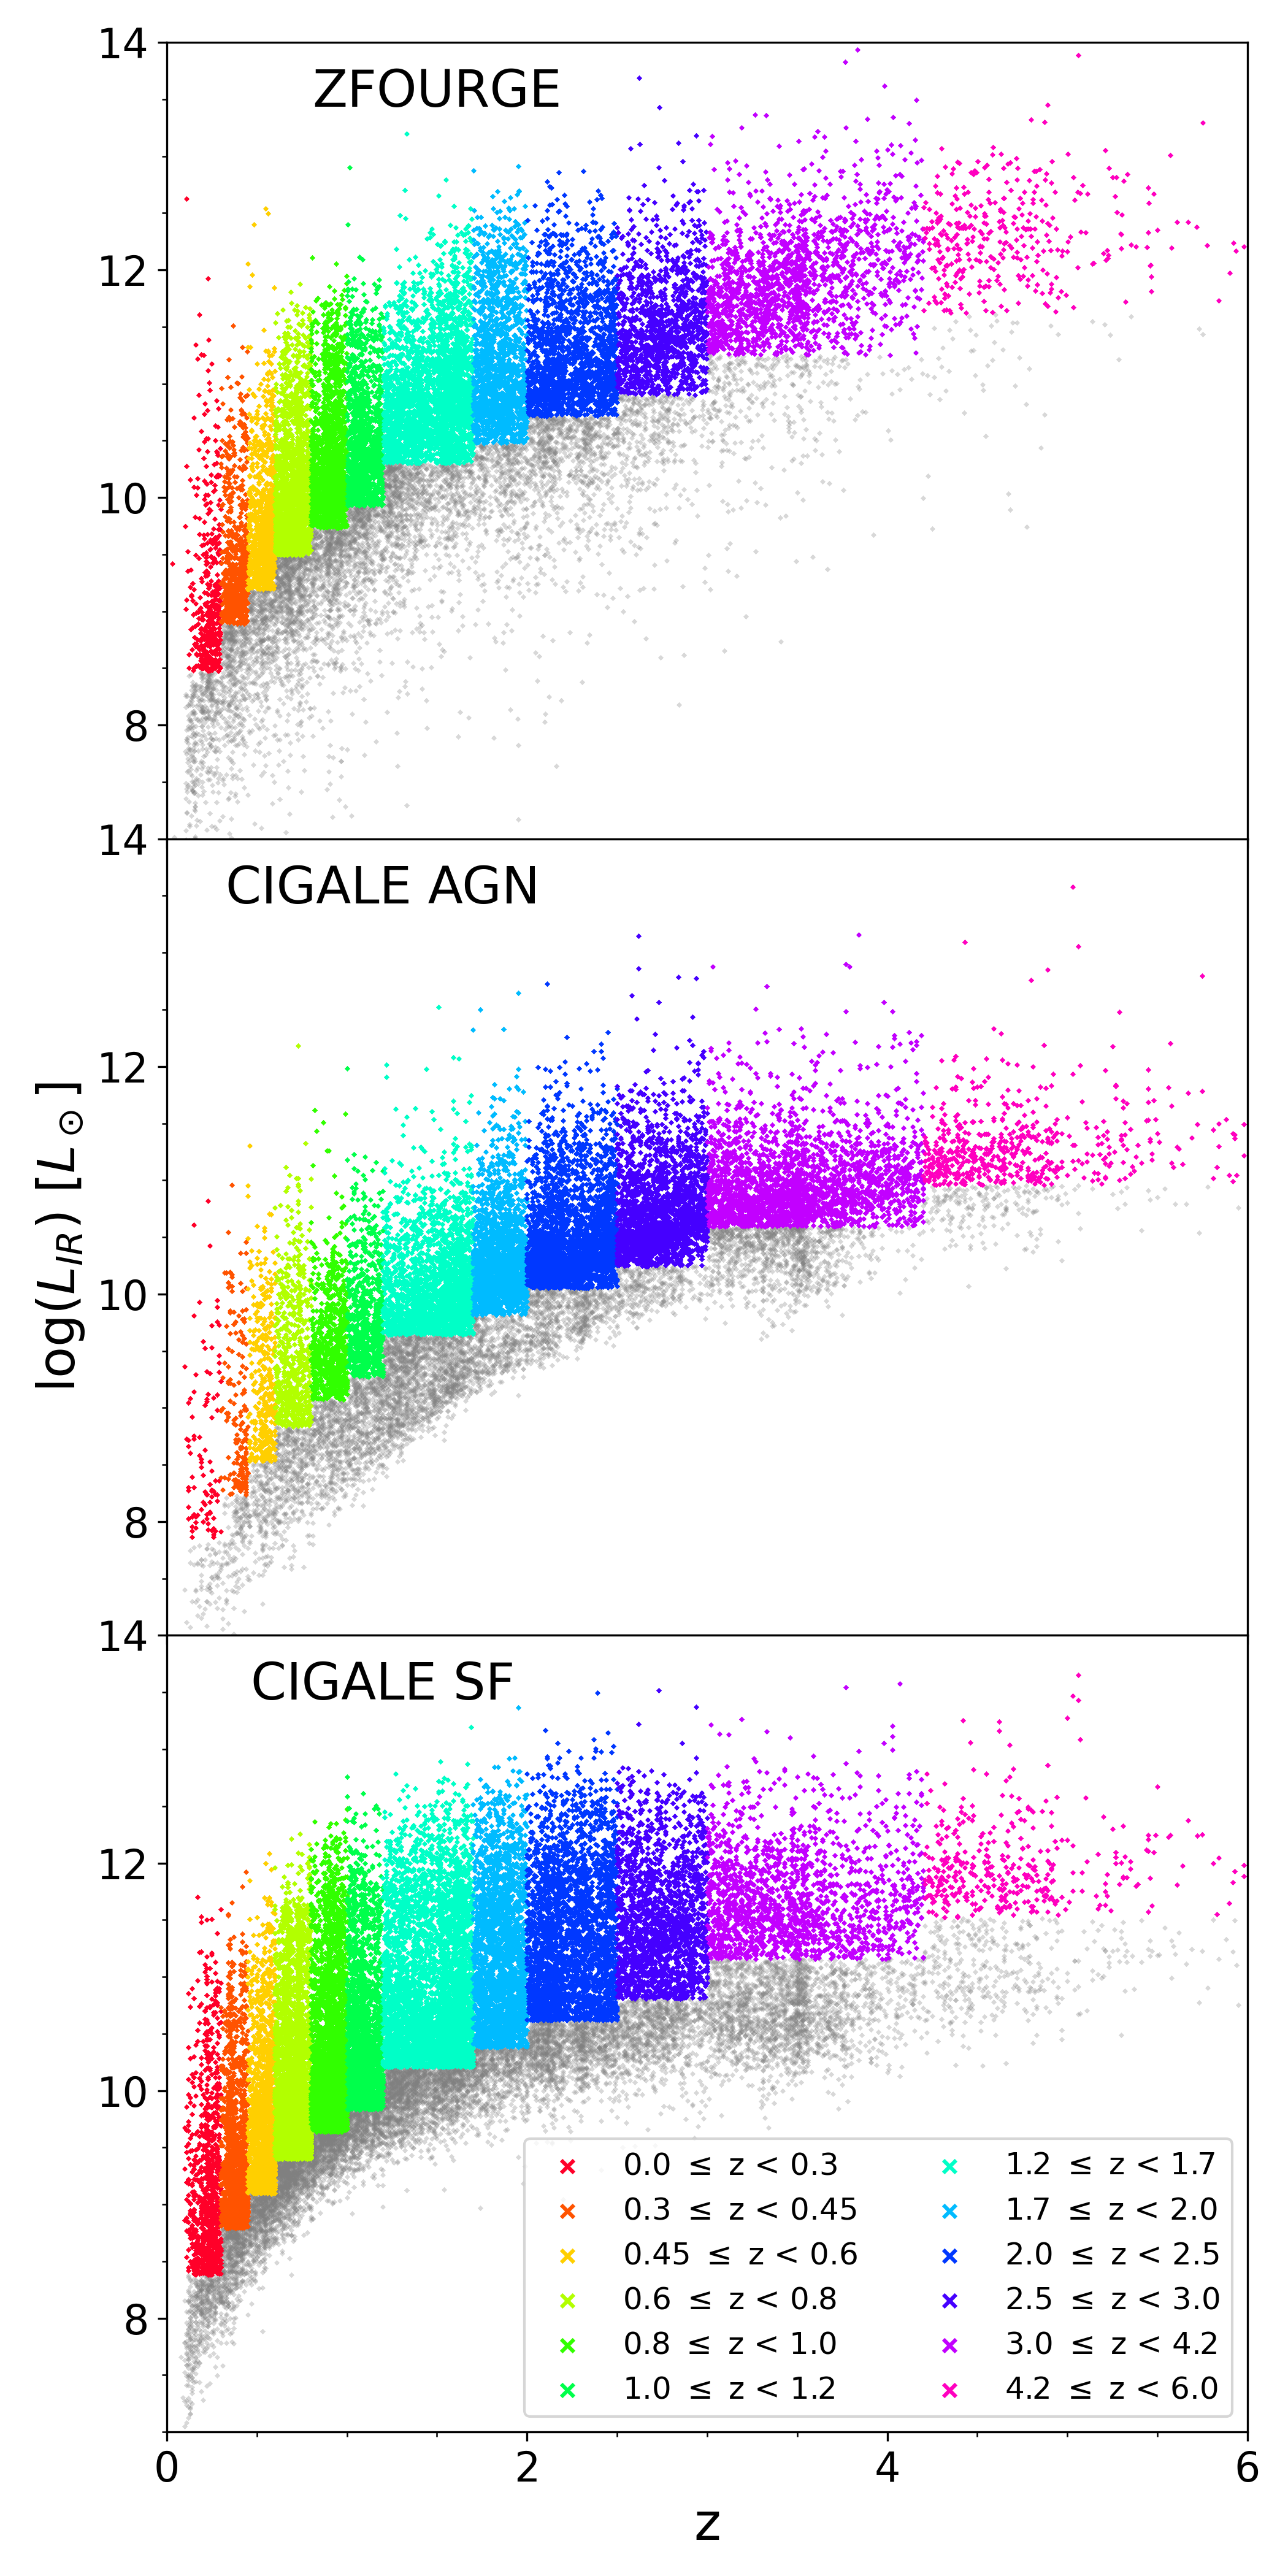
\includegraphics[width=0.48\textwidth]{Figures/LIR_vs_Z.png}
    \caption{Luminosity-redshift distributions of (top) the ZFOURGE bolometric $8-1000\mu m$ IR luminosity, (middle) the CIGALE AGN luminosity, and (bottom) the CIGALE SF luminosity. Sources are coloured by redshift bin or coloured grey if removed as described in section \ref{Sec: Sample Selection}}
    \label{Fig: ZF Lum vs z}
\end{figure}

% \textcolor{red}{Paragraph on population bias of missing data. The faint end is impacted? other NIR surveys like ultravista, 3dhst, did they do luminosity funcitons and did they address it? We are limited by our survey, so there is a gap at that end. But people miss things in LFs all the time, and were just going to miss these.}

% \textcolor{red}{is this paragraph even necessary? I feel like it could be deleted entirely.} We use the UVJ colour-colour diagram to differentiate between quiescent and star-forming galaxies by selecting a quiescent galaxy mask with equation \ref{EQ: UVJ} \citep{cowley_zfourge_2016}. \textcolor{red}{better reference?}. Where U, V, \& J are the rest-frame Johnson U, V and 2MASS J filters respectively. \citep{straatman_fourstar_2016}. Star-forming galaxies are selected by taking the inverse of the quiescent galaxy mask.

% \begin{equation}
%     \label{EQ: UVJ}
%     \begin{split}
%         & U-V > 1.3, \\
%         & V-J < 1.6, \\
%         & U-V > 0.88 \times (V-J) + 0.59
%     \end{split}
% \end{equation}